% !TEX root = ../notes_unsupervisedlearning.tex
% Chapter 8: Self-Supervised Learning
%%%%%%%%%%%%%%%%%%%%%%%%%%%%%%%%%%%%%%%%%%%%%%%%%%%%%%%%%%%%%%%%%%%%%%

\chapter{Self-Supervised Learning}\index{Self-Supervised Learning}\index{SimCLR}\index{BERT}
\newthought{Labels are expensive. Let data supervise itself.}

%═══════════════════════════════════════════════════════════════════════
% BLOCK 1: INTRODUCTION
%═══════════════════════════════════════════════════════════════════════

\section{The Why}

\marginnote{Unlabeled data is abundant; labels are scarce and expensive.}

The deep learning revolution was built on labeled data. But labeling is expensive:
\begin{itemize}
    \item ImageNet: 14 million images, years of labeling effort
    \item Medical imaging: \$50--500 per expert annotation
    \item Autonomous driving: hours per scene for 3D labeling
\end{itemize}

Meanwhile, unlabeled data is virtually unlimited: the internet has billions of images, trillions of text tokens, endless video.

\textbf{Self-supervised learning} extracts supervision from the data itself by designing \textbf{pretext tasks}---auxiliary tasks whose labels come for free from data structure.

\begin{figure}[h]
\centering
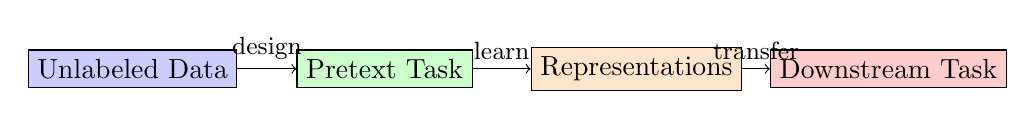
\begin{tikzpicture}[node distance=1.2cm]
    \node[draw, rectangle, fill=blue!20] (data) {Unlabeled Data};
    \node[draw, rectangle, right of=data, xshift=2cm, fill=green!20] (pretext) {Pretext Task};
    \node[draw, rectangle, right of=pretext, xshift=2cm, fill=orange!20] (repr) {Representations};
    \node[draw, rectangle, right of=repr, xshift=2cm, fill=red!20] (down) {Downstream Task};

    \draw[->] (data) -- node[above] {\small design} (pretext);
    \draw[->] (pretext) -- node[above] {\small learn} (repr);
    \draw[->] (repr) -- node[above] {\small transfer} (down);
\end{tikzpicture}
\caption{Self-supervised learning pipeline: design pretext task $\to$ learn representations $\to$ transfer to downstream tasks.}
\end{figure}

\subsection{Hands-On Experience}

Consider an image. Design a pretext task:
\begin{enumerate}
    \item Rotate the image by $0°, 90°, 180°, 270°$. Train a classifier to predict rotation.
    \item Split into patches, shuffle them. Train to predict correct arrangement.
    \item Convert to grayscale. Train to predict original colors.
\end{enumerate}

\marginnote{The pretext task should be hard enough to require understanding image structure.}

Each task forces the model to understand image structure---object shapes, semantics, texture---to succeed. The learned features transfer to real tasks like classification.

\subsection{Learning Objectives}

After this lecture, you will be able to:
\begin{enumerate}
    \item Design pretext tasks that yield useful representations
    \item Implement contrastive learning (SimCLR, MoCo)
    \item Explain non-contrastive methods (BYOL, SimSiam) and why they don't collapse
    \item Apply masked prediction for vision (MAE) and language (BERT)
    \item Choose appropriate self-supervised methods for different modalities
\end{enumerate}

%═══════════════════════════════════════════════════════════════════════
% BLOCK 2: MAIN THEORY
%═══════════════════════════════════════════════════════════════════════

\section{Pretext Tasks}

\marginnote{A pretext task creates pseudo-labels from data structure.}

Early self-supervised methods designed clever pretext tasks:

\begin{table}[h]
\centering
\begin{tabular}{ll}
\toprule
\textbf{Task} & \textbf{Supervision Signal} \\
\midrule
Rotation prediction & Predict rotation angle (0/90/180/270) \\
Jigsaw puzzle & Predict patch permutation \\
Colorization & Predict colors from grayscale \\
Inpainting & Predict missing image regions \\
Context prediction & Predict relative position of patches \\
\bottomrule
\end{tabular}
\caption{Classic pretext tasks for images}
\end{table}

\textbf{Limitation}: Pretext task performance doesn't always correlate with downstream task performance. We need more principled approaches.


\section{Contrastive Learning}

\marginnote{Core idea: pull similar things together, push different things apart.}

\textbf{Contrastive learning} learns representations by:
\begin{enumerate}
    \item Creating \textbf{positive pairs}: augmented views of the same sample
    \item Creating \textbf{negative pairs}: views of different samples
    \item Training to distinguish positives from negatives
\end{enumerate}

\subsection{InfoNCE Loss}

Given an anchor $x$, positive $x^+$, and negatives $\{x^-_k\}$:

\begin{equation}
    \mathcal{L}_{\text{InfoNCE}} = -\log \frac{\exp(\text{sim}(z, z^+) / \tau)}{\exp(\text{sim}(z, z^+) / \tau) + \sum_k \exp(\text{sim}(z, z^-_k) / \tau)}
\end{equation}

where $\text{sim}(u, v) = u \cdot v / (\|u\| \|v\|)$ is cosine similarity and $\tau$ is temperature.

\begin{figure}[h]
\centering
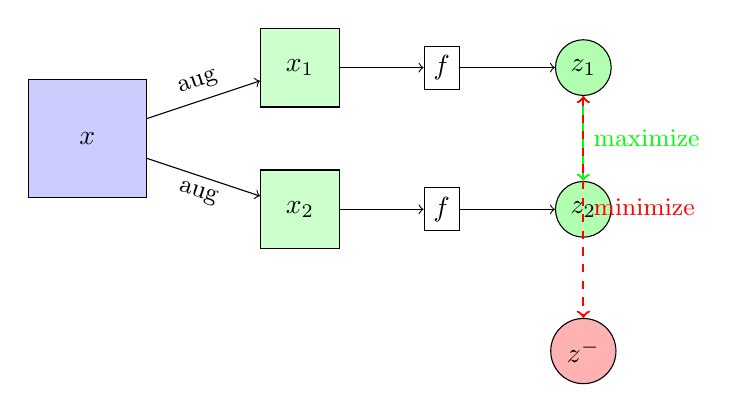
\begin{tikzpicture}[scale=0.9]
    % Original image
    \node[draw, rectangle, minimum width=1.5cm, minimum height=1.5cm, fill=blue!20] (orig) at (0,0) {$x$};

    % Augmentations
    \node[draw, rectangle, minimum width=1cm, minimum height=1cm, fill=green!20] (aug1) at (3,1) {$x_1$};
    \node[draw, rectangle, minimum width=1cm, minimum height=1cm, fill=green!20] (aug2) at (3,-1) {$x_2$};

    % Encoders
    \node[draw, rectangle] (enc1) at (5,1) {$f$};
    \node[draw, rectangle] (enc2) at (5,-1) {$f$};

    % Representations
    \node[draw, circle, fill=green!30] (z1) at (7,1) {$z_1$};
    \node[draw, circle, fill=green!30] (z2) at (7,-1) {$z_2$};

    % Arrows
    \draw[->] (orig) -- node[above, sloped] {\small aug} (aug1);
    \draw[->] (orig) -- node[below, sloped] {\small aug} (aug2);
    \draw[->] (aug1) -- (enc1);
    \draw[->] (aug2) -- (enc2);
    \draw[->] (enc1) -- (z1);
    \draw[->] (enc2) -- (z2);

    % Similarity
    \draw[<->, green, thick] (z1) -- node[right] {\small maximize} (z2);

    % Negative
    \node[draw, circle, fill=red!30] (zneg) at (7,-3) {$z^-$};
    \draw[<->, red, thick, dashed] (z1) -- node[right] {\small minimize} (zneg);
\end{tikzpicture}
\caption{Contrastive learning: augmented views of same image should have similar representations.}
\end{figure}


\section{SimCLR}

\marginnote{SimCLR: Simple Contrastive Learning of Visual Representations (Chen et al., 2020)}

\textbf{SimCLR} is a simple and effective contrastive framework:

\begin{algorithm}[H]
\caption{SimCLR}
\begin{algorithmic}[1]
\For{each minibatch of $N$ images}
    \State Generate $2N$ augmented views (2 per image)
    \For{each positive pair $(i, j)$}
        \State $z_i = g(f(x_i))$ \Comment{Encoder + projection head}
        \State $z_j = g(f(x_j))$
        \State Treat other $2(N-1)$ views as negatives
        \State Compute InfoNCE loss
    \EndFor
\EndFor
\end{algorithmic}
\end{algorithm}

\textbf{Key ingredients}:
\begin{enumerate}
    \item \textbf{Strong augmentations}: Random crop, color jitter, Gaussian blur, etc.
    \item \textbf{Projection head}: MLP after encoder; discarded after training
    \item \textbf{Large batch sizes}: More negatives $\to$ better performance (4096+)
    \item \textbf{Temperature}: $\tau = 0.1$ works well
\end{enumerate}


\section{MoCo}

\marginnote{MoCo: Momentum Contrast (He et al., 2020)}

SimCLR needs huge batches for enough negatives. \textbf{MoCo} uses a \textbf{queue} of negatives:

\begin{itemize}
    \item Maintain a queue of recent embeddings as negatives
    \item Use a \textbf{momentum encoder} (slowly updated copy) for consistency
    \item Update: $\theta_k \gets m \theta_k + (1-m) \theta_q$ where $m = 0.999$
\end{itemize}

Benefits: Works with small batches (256), memory-efficient.


\section{Non-Contrastive Methods}

\marginnote{Surprising finding: you don't need negatives!}

\subsection{BYOL: Bootstrap Your Own Latent}

\textbf{BYOL} learns without negative pairs:
\begin{enumerate}
    \item Online network: encoder $\to$ projector $\to$ predictor
    \item Target network: encoder $\to$ projector (momentum-updated)
    \item Loss: MSE between online prediction and target projection
\end{enumerate}

\begin{equation}
    \mathcal{L}_{\text{BYOL}} = \|q_\theta(z_1) - \text{sg}(z'_2)\|^2
\end{equation}

where $\text{sg}$ means stop-gradient (no backprop through target).

\subsection{SimSiam: Simple Siamese}

\textbf{SimSiam} is even simpler---no momentum encoder:
\begin{equation}
    \mathcal{L} = -\frac{1}{2} \left( \text{sim}(p_1, \text{sg}(z_2)) + \text{sim}(p_2, \text{sg}(z_1)) \right)
\end{equation}

\subsection{Why Don't They Collapse?}

\marginnote{Without negatives, why doesn't everything map to a constant?}

Several hypotheses:
\begin{itemize}
    \item \textbf{Asymmetry}: Predictor network breaks symmetry
    \item \textbf{Stop-gradient}: Prevents both branches from collapsing together
    \item \textbf{BatchNorm}: Implicitly creates contrastive signal within batch
\end{itemize}


\section{Masked Prediction}

\marginnote{Mask part of the input; predict the masked part.}

\subsection{BERT: Masked Language Modeling}

\begin{enumerate}
    \item Mask 15\% of tokens randomly
    \item Of masked: 80\% [MASK], 10\% random, 10\% unchanged
    \item Train to predict original tokens
\end{enumerate}

\begin{equation}
    \mathcal{L}_{\text{MLM}} = -\sum_{i \in \text{masked}} \log p(x_i | x_{\backslash i})
\end{equation}

\subsection{MAE: Masked Autoencoders}

\marginnote{MAE: Mask 75\% of image patches, reconstruct pixels.}

For vision:
\begin{enumerate}
    \item Divide image into patches (e.g., 16×16)
    \item Mask 75\% of patches randomly
    \item Encode visible patches with transformer
    \item Decode (with mask tokens) to reconstruct pixels
\end{enumerate}

\begin{figure}[h]
\centering
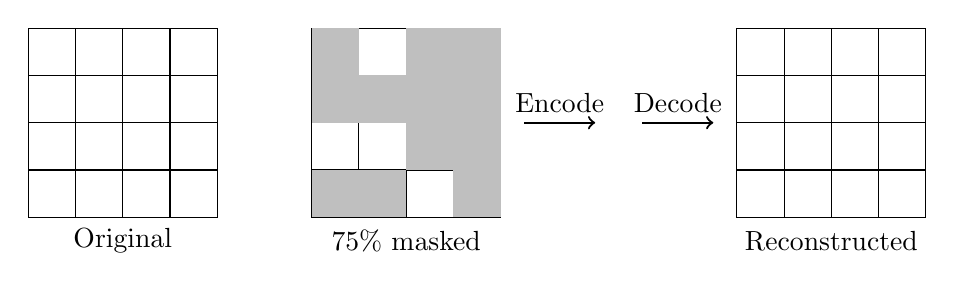
\begin{tikzpicture}[scale=0.6]
    % Original image grid
    \foreach \i in {0,1,2,3} {
        \foreach \j in {0,1,2,3} {
            \draw (\i,\j) rectangle (\i+1,\j+1);
        }
    }
    \node at (2,-0.5) {Original};

    % Masked version
    \begin{scope}[xshift=6cm]
    \foreach \i in {0,1,2,3} {
        \foreach \j in {0,1,2,3} {
            \draw (\i,\j) rectangle (\i+1,\j+1);
        }
    }
    % Fill masked patches
    \fill[gray!50] (0,0) rectangle (1,1);
    \fill[gray!50] (1,0) rectangle (2,1);
    \fill[gray!50] (2,1) rectangle (3,2);
    \fill[gray!50] (0,2) rectangle (1,3);
    \fill[gray!50] (1,2) rectangle (2,3);
    \fill[gray!50] (2,2) rectangle (3,3);
    \fill[gray!50] (3,2) rectangle (4,3);
    \fill[gray!50] (0,3) rectangle (1,4);
    \fill[gray!50] (2,3) rectangle (3,4);
    \fill[gray!50] (3,3) rectangle (4,4);
    \fill[gray!50] (3,0) rectangle (4,1);
    \fill[gray!50] (3,1) rectangle (4,2);
    \node at (2,-0.5) {75\% masked};
    \end{scope}

    % Arrow
    \draw[->, thick] (10.5,2) -- (12,2) node[midway, above] {Encode};
    \draw[->, thick] (13,2) -- (14.5,2) node[midway, above] {Decode};

    % Reconstructed
    \begin{scope}[xshift=15cm]
    \foreach \i in {0,1,2,3} {
        \foreach \j in {0,1,2,3} {
            \draw (\i,\j) rectangle (\i+1,\j+1);
        }
    }
    \node at (2,-0.5) {Reconstructed};
    \end{scope}
\end{tikzpicture}
\caption{MAE: mask most patches, reconstruct pixels.}
\end{figure}

\subsection{Data2Vec}

Generalizes masked prediction across modalities (vision, speech, text) using a single framework with teacher-student distillation.


\section{Cross-Modal Self-Supervision}

\marginnote{CLIP: learn joint image-text representations from web data.}

\textbf{CLIP} (Contrastive Language-Image Pre-training):
\begin{itemize}
    \item Train on 400M image-caption pairs from the web
    \item Contrastive loss: match images with their captions
    \item Result: powerful zero-shot transfer to new tasks
\end{itemize}

This bridges to next chapter on zero-shot learning.


%═══════════════════════════════════════════════════════════════════════
% BLOCK 3: STUDENT ACTIVATION
%═══════════════════════════════════════════════════════════════════════

\section{Examples \& Exercises}

\subsection{Exercise 1: Design a Pretext Task}

Propose a self-supervised pretext task for:
\begin{enumerate}
    \item Audio data (e.g., speech recordings)
    \item Time series (e.g., sensor readings)
    \item Graphs (e.g., molecular structures)
\end{enumerate}

\textbf{Solutions}:
\begin{enumerate}
    \item Audio: Predict next audio frame, predict speaker identity, contrastive on time-shifted clips
    \item Time series: Predict future values, contrastive on temporal augmentations, predict transformations
    \item Graphs: Mask nodes/edges, contrastive on graph augmentations (drop edges, mask features)
\end{enumerate}

\subsection{Exercise 2: InfoNCE Loss}

Given embeddings with cosine similarities:
\begin{itemize}
    \item $\text{sim}(z, z^+) = 0.9$
    \item $\text{sim}(z, z^-_1) = 0.3$, $\text{sim}(z, z^-_2) = 0.1$
\end{itemize}

Compute InfoNCE loss with $\tau = 0.5$.

\textbf{Solution}:
\begin{align*}
    \mathcal{L} &= -\log \frac{e^{0.9/0.5}}{e^{0.9/0.5} + e^{0.3/0.5} + e^{0.1/0.5}} \\
    &= -\log \frac{e^{1.8}}{e^{1.8} + e^{0.6} + e^{0.2}} \\
    &= -\log \frac{6.05}{6.05 + 1.82 + 1.22} \approx -\log(0.66) \approx 0.41
\end{align*}

\subsection{Exercise 3: Augmentation Ablation}

Why is random cropping important in SimCLR? What would happen without it?

\textbf{Solution}: Random cropping forces the model to learn features invariant to position and scale. Without it, two augmentations of the same image might share only color information, leading to representations that encode color but not object identity.


\section{Self-Reflection \& Recap}

\subsection{Reflection Questions}
\begin{enumerate}
    \item Why is the projection head discarded after training in SimCLR?
    \begin{quote}
        \textit{The projection head removes information useful for contrastive learning but not for downstream tasks. The encoder before the head retains more general features.}
    \end{quote}

    \item What prevents collapse in non-contrastive methods?
    \begin{quote}
        \textit{Asymmetry (predictor network) and stop-gradient break the symmetry that would allow both branches to collapse to a constant.}
    \end{quote}
\end{enumerate}

\subsection{Key Concepts}
\begin{itemize}
    \item Self-supervision creates labels from data structure
    \item \textbf{Contrastive}: pull positives together, push negatives apart
    \item \textbf{Non-contrastive}: works without negatives (BYOL, SimSiam)
    \item \textbf{Masked prediction}: reconstruct missing information (BERT, MAE)
    \item Augmentations are crucial for defining what should be invariant
\end{itemize}

\subsection{Next Chapter Teaser}
\marginnote{Teaser: From learning to transferring}
\newthought{We can now learn powerful representations without labels.} But can we use these representations for tasks we never trained for? The next chapter explores \textbf{zero-shot and few-shot learning}---leveraging pre-trained knowledge for new tasks with minimal or no examples.
